%==============================================================================
%  MATH 231 -- Linear Algebra I (Queens College, Fall 2026)
%  MATRIX UNIT, PART 5 -- Projection Matrices and the Direct Sum
%
%  Section numbering runs CONTINUOUSLY across the parts of the matrix unit;
%  see Part 2's header for the full map.  This part is Sections 26-29, hence
%  \setcounter{section}{25}.
%
%  STATUS: complete.  Sections 26-29.  Written from the plan in
%  plan/MATH231_remaining_units_plan.tex (2026-10-25).
%
%  AUDIENCE: distributed to students.  No instructor-facing apparatus.
%
%  WHAT THE INSTRUCTOR SPECIFIED, AND WHERE IT IS.
%   - The projection matrix as "the first example derived from the
%     projection formula (projecting vectors in R^2 onto a 1-dimensional
%     subspace)": Sec. 26.2, from the vector unit's Sec. 12.4 formula.
%   - A projection matrix defined as an idempotent matrix, with idempotency
%     defined "intuitively and briefly": Sec. 27.1-27.2.
%   - The complementary projection, which for the 1-D case is the orthogonal
%     projection with respect to a vector v: Sec. 28.3 (I - P_u = P_v for
%     v perpendicular to u in R^2).  The orthogonal projection matrix
%     defined from the projection of one vector onto another: Sec. 26.2 and
%     its restatement for v in Sec. 28.3.
%   - The direct sum, intuitively, from span{u} and span{v} with u, v
%     orthogonal, using P and its complement: Sec. 29.1-29.3.
%   - The Householder reflector, derived in R^2 as in class (Nov 3, 2026):
%     reflect u onto the x-axis across the line through the average
%     (centroid) m = (u + ||u|| e_1)/2, which gives H = 2vv' - I_2 with
%     v = m/||m||: Sec. 28.5-28.6.  Sec. 28.7 adds the properties, the
%     first-column check, the negative-x-axis exception, and the usual form
%     I - 2ww' (the form Part 11 Sec. 58.4 cites).  Kept inside Sec. 28 at
%     the instructor's choice, so no later section number moves.
%
%  NOTATION (plan N3).  The complementary projection is written I - P_u.
%  The letter Q is reserved for orthogonal matrices and the QR factorization
%  (Part 11).  NB the held-back Homework 3 Part G problems write Q_u for
%  I - P_u; rename when assigning them.
%
%  PROJECTION SUBSCRIPT CONVENTION, as in the vector unit's Sec. 12.4:
%  proj_u(v) projects v ONTO u, and P_u is the matrix of v -> proj_u(v).
%
%  [proposed in the plan, included:] the oblique (non-symmetric) idempotent
%  [1 1; 0 0] in Sec. 27.3, the definition of an ORTHOGONAL projection
%  (P^2 = P and P' = P) with the short proof that the residual is
%  perpendicular, the reflection 2P_u - I in Sec. 28.4, and the oblique
%  direct sum in Sec. 29.4.  Delete freely; nothing later depends on 27.3 or
%  29.4.  Sec. 27.4 (orthogonal projection) IS used by Part 9 and Part 10.
%
%  Compile with pdflatex or tectonic (standard TeX Live packages only; uses
%  tikz).
%==============================================================================
\documentclass[11pt]{article}

\usepackage[margin=1in]{geometry}
\usepackage{amsmath,amssymb,amsthm}
\usepackage[dvipsnames]{xcolor}
\usepackage{enumitem}
\usepackage{booktabs}
\usepackage{array}
\usepackage[hidelinks]{hyperref}
\usepackage{titlesec}
\usepackage{needspace}
\usepackage{tikz}
\usetikzlibrary{arrows.meta}

%------------------------------------------------------------------ style ----
\titleformat{\section}{\large\bfseries\sffamily}{\thesection.}{0.6em}{}
\titleformat{\subsection}{\normalsize\bfseries\sffamily}{\thesubsection.}{0.5em}{}
\titlespacing*{\section}{0pt}{14pt}{6pt}
\setlength{\emergencystretch}{3em}

\theoremstyle{plain}
\newtheorem{thm}{Theorem}[section]
\newtheorem{lem}[thm]{Lemma}
\newtheorem{cor}[thm]{Corollary}

\theoremstyle{definition}
\newtheorem{defn}{Definition}[section]
\newtheorem{ex}{Example}[section]
\theoremstyle{remark}
\newtheorem*{rmk}{Remark}
\newtheorem*{warn}{A common confusion}

\newcommand{\lookahead}{\par\smallskip\noindent
  \textbf{\sffamily\textcolor{RoyalBlue}{Looking ahead.}}\ \ignorespaces}
\newcommand{\lookback}[1][the vector unit]{\par\smallskip\noindent
  \textbf{\sffamily\textcolor{ForestGreen}{From #1.}}\ \ignorespaces}

%--------------------------------------------------------------- notation ----
\newcommand{\R}{\mathbb{R}}
\newcommand{\vc}[1]{\mathbf{#1}}
\newcommand{\mt}[1]{\mathbf{#1}}
\newcommand{\norm}[1]{\lVert #1\rVert}
\newcommand{\T}{^{\mathsf{T}}}
\newcommand{\proj}[2]{\operatorname{proj}_{#1}(#2)}
\newcommand{\colsp}[1]{\operatorname{col}[#1]}
\DeclareMathOperator{\spanop}{span}
\DeclareMathOperator{\diagop}{diag}
\DeclareMathOperator{\rank}{rank}

%------------------------------------------------------------- tikz helpers --
\tikzset{
  vecarr/.style   = {-{Stealth[length=2.6mm,width=2.0mm]},very thick},
  thinarr/.style  = {-{Stealth[length=2.2mm,width=1.7mm]},thick},
  axisline/.style = {->,gray!75,thin}
}

\title{\vspace{-1.2cm}\textbf{\sffamily MATH 231 -- Linear Algebra I}\\[4pt]
       {\large\sffamily The Matrix Unit, Part 5 \textbullet\ Projection
        Matrices and the Direct Sum}\\[2pt]
       {\normalsize\sffamily Kiely Hall 326 \textbullet\
        Instructor: Kevin Bedoya}}
\author{}
\date{}

\begin{document}
\setcounter{section}{25}  % this part opens at Section 26; see the header note
\maketitle
\vspace{-1.6cm}

\noindent\textbf{About this document.} This is Part 5 of the matrix unit,
Sections 26--29. Section numbers run continuously through the unit (Part 2's
opening table lists them all). References into the vector unit always name it.

\medskip
\noindent\textbf{Assumed.} From the vector unit: the projection
$\proj{\vc{u}}{\vc{v}}$ and the orthogonal piece $\vc{v}-\proj{\vc{u}}{\vc{v}}$
(\S12.4--\S12.6), orthogonal vectors being independent (\S21.2), and the
Pythagorean identity (\S23). From this unit: the inner and outer products
$\vc{u}\T\vc{v}$ and $\vc{u}\vc{v}\T$ (\S7), the laws M1--M6 (\S8.4), the
projection onto the $x$-axis (\S19.3), and the reflections of \S19--\S21.

\medskip
\noindent\textbf{What you should be able to do afterwards.} Write down the
matrix that projects onto a given line and use it; say what idempotent means and
check whether a matrix is a projection; distinguish an orthogonal projection
from a slanted one; build the complementary projection and identify it in
$\R^{2}$ as the projection onto the perpendicular line; build a reflection from
a projection; build the Householder reflector that sends a vector onto the
$x$-axis; and split a vector into its pieces along a direct sum.

%==============================================================================
\section{The projection matrix onto a line}
%==============================================================================

%------------------------------------------------------------------------------
\subsection{The formula we already have}
%------------------------------------------------------------------------------
\lookback For a nonzero vector $\vc{u}$, the projection of $\vc{v}$ onto
$\vc{u}$ is the shadow $\vc{v}$ casts on the line through $\vc{u}$ when the
light falls perpendicular to that line (\S12.4):
\[
  \proj{\vc{u}}{\vc{v}}=\frac{\vc{u}\cdot\vc{v}}{\vc{u}\cdot\vc{u}}\,\vc{u}.
\]
The subscript names the vector projected \emph{onto}. What is left over,
$\vc{v}-\proj{\vc{u}}{\vc{v}}$, is orthogonal to $\vc{u}$ (\S12.6).

The formula takes a vector $\vc{v}$ and returns a vector. It is linear in
$\vc{v}$: the numerator $\vc{u}\cdot\vc{v}$ is, and nothing else depends on
$\vc{v}$. So by \S13.3 there is a matrix that does it. This section finds it, not
from where it sends $\vc{e}_1$ and $\vc{e}_2$, but straight from the formula.

%------------------------------------------------------------------------------
\subsection{From the formula to the matrix}
%------------------------------------------------------------------------------
Three moves, each one a law already proved.
\begin{enumerate}[label=(\arabic*),leftmargin=2em,itemsep=4pt]
  \item Write the dot products as matrix products, $\vc{u}\cdot\vc{v}=\vc{u}\T\vc{v}$
        (\S7.1):
        \[\proj{\vc{u}}{\vc{v}}=\frac{\vc{u}\T\vc{v}}{\vc{u}\T\vc{u}}\,\vc{u}.\]
  \item The fraction is a number, so it can be written on the right of $\vc{u}$
        instead of the left (M4):
        \[\proj{\vc{u}}{\vc{v}}=\vc{u}\,\frac{\vc{u}\T\vc{v}}{\vc{u}\T\vc{u}}
          =\frac{1}{\vc{u}\T\vc{u}}\;\vc{u}\,(\vc{u}\T\vc{v}).\]
  \item Regroup with associativity (M1), reading $\vc{u}$ as $n\times1$,
        $\vc{u}\T$ as $1\times n$ and $\vc{v}$ as $n\times1$:
        $\vc{u}(\vc{u}\T\vc{v})=(\vc{u}\vc{u}\T)\vc{v}$. So
        \[\proj{\vc{u}}{\vc{v}}=\frac{\vc{u}\vc{u}\T}{\vc{u}\T\vc{u}}\;\vc{v}.\]
\end{enumerate}
The thing multiplying $\vc{v}$ no longer depends on $\vc{v}$. It is a matrix.

\begin{defn}[Projection matrix onto a line]
For a nonzero $\vc{u}\in\R^{n}$, the \textbf{projection matrix onto the line
$\spanop\{\vc{u}\}$} is
\[
  \boxed{\;\mt{P}_{\vc{u}}=\frac{\vc{u}\vc{u}\T}{\vc{u}\T\vc{u}}\;}
  \qquad\text{so that}\qquad
  \mt{P}_{\vc{u}}\vc{v}=\proj{\vc{u}}{\vc{v}}\ \text{ for every }\vc{v}.
\]
It is the outer product $\vc{u}\vc{u}\T$ (\S7.2), an $n\times n$ matrix, divided
by the number $\vc{u}\T\vc{u}=\norm{\vc{u}}^{2}$.
\end{defn}

\noindent The matrix depends only on the \emph{line}, not on which vector along
it was chosen. Replacing $\vc{u}$ by $c\vc{u}$ multiplies the top by $c^{2}$ and
the bottom by $c^{2}$. In particular, for a unit vector $\hat{\vc{u}}$ the
denominator is $1$ and $\mt{P}_{\vc{u}}=\hat{\vc{u}}\hat{\vc{u}}\T$.

%------------------------------------------------------------------------------
\subsection{Examples}
%------------------------------------------------------------------------------
\begin{ex}
\label{ex:proj}
\leavevmode
\begin{enumerate}[label=(\alph*),leftmargin=2em,itemsep=4pt]
  \item $\vc{u}=\vc{e}_1=[\,1,0\,]$: $\vc{u}\vc{u}\T=\begin{bmatrix}1&0\\0&0\end{bmatrix}$
        and $\vc{u}\T\vc{u}=1$, so $\mt{P}_{\vc{e}_1}=\diagop(1,0)$, the projection
        onto the $x$-axis that \S19.3 built from $\vc{e}_1$ and $\vc{e}_2$.
        The two constructions agree.
  \item $\vc{u}=[\,1,1\,]$: $\mt{P}_{\vc{u}}=\frac12\begin{bmatrix}1&1\\1&1\end{bmatrix}$.
        For $\vc{v}=[\,3,1\,]$, $\mt{P}_{\vc{u}}\vc{v}=\frac12[\,4,4\,]=[\,2,2\,]$.
        The formula agrees: $\frac{\vc{u}\cdot\vc{v}}{\vc{u}\cdot\vc{u}}\vc{u}=\frac42[\,1,1\,]$.
  \item $\vc{u}=[\,2,1\,]$: $\mt{P}_{\vc{u}}=\frac15\begin{bmatrix}4&2\\2&1\end{bmatrix}$.
        For $\vc{v}=[\,1,3\,]$, $\mt{P}_{\vc{u}}\vc{v}=\frac15[\,10,5\,]=[\,2,1\,]$,
        and the leftover $\vc{v}-\mt{P}_{\vc{u}}\vc{v}=[\,-1,2\,]$ is orthogonal to
        $\vc{u}$. This is the picture below.
  \item In $\R^{3}$, $\vc{u}=[\,1,1,1\,]$:
        $\mt{P}_{\vc{u}}=\frac13\begin{bmatrix}1&1&1\\1&1&1\\1&1&1\end{bmatrix}$,
        and $\mt{P}_{\vc{u}}\vc{v}$ replaces every entry of $\vc{v}$ by the average
        of the entries: $\mt{P}_{\vc{u}}[\,1,2,6\,]=[\,3,3,3\,]$.
\end{enumerate}
\end{ex}

\begin{center}
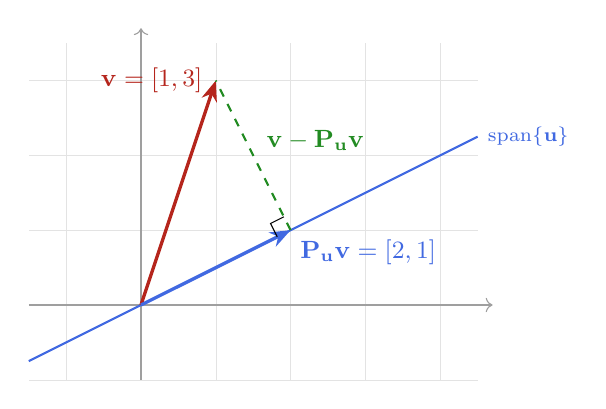
\begin{tikzpicture}[scale=0.95]
  \draw[step=1cm,gray!22,very thin] (-1.5,-1) grid (4.5,3.5);
  \draw[axisline] (-1.5,0) -- (4.7,0);
  \draw[axisline] (0,-1) -- (0,3.7);
  \draw[RoyalBlue,thick] (-1.5,-0.75) -- (4.5,2.25)
       node[right,font=\scriptsize]{$\spanop\{\vc{u}\}$};
  \draw[vecarr,BrickRed] (0,0) -- (1,3);
  \node[left,font=\small,BrickRed] at (0.95,3) {$\vc{v}=[1,3]$};
  \draw[vecarr,RoyalBlue] (0,0) -- (2,1);
  \node[below right,font=\small,RoyalBlue] at (2,1) {$\mt{P}_{\vc{u}}\vc{v}=[2,1]$};
  \draw[dashed,thick,ForestGreen] (2,1) -- (1,3);
  \node[right,font=\small,ForestGreen] at (1.55,2.2) {$\vc{v}-\mt{P}_{\vc{u}}\vc{v}$};
  \draw (1.821,0.9105) -- (1.7315,1.0895) -- (1.9105,1.179);
\end{tikzpicture}
\end{center}

%------------------------------------------------------------------------------
\subsection{The structure of \texorpdfstring{$\mt{P}_{\vc{u}}$}{P\_u}}
%------------------------------------------------------------------------------
Read off the definition:
\begin{itemize}[leftmargin=1.4em,itemsep=3pt]
  \item \textbf{Symmetric.} $(\vc{u}\vc{u}\T)\T=(\vc{u}\T)\T\vc{u}\T=\vc{u}\vc{u}\T$
        by M6.
  \item \textbf{Column space the line.} Column $j$ of $\vc{u}\vc{u}\T$ is
        $u_j\vc{u}$, a multiple of $\vc{u}$. So $\colsp{\mt{P}_{\vc{u}}}=\spanop\{\vc{u}\}$
        and $\rank\mt{P}_{\vc{u}}=1$. In $\R^{2}$ that means
        $\det\mt{P}_{\vc{u}}=0$ (\S14.2); e.g.\ $\frac15(4\cdot1-2\cdot2)=0$.
  \item \textbf{The line is kept.} $\mt{P}_{\vc{u}}\vc{u}=\vc{u}\,\frac{\vc{u}\T\vc{u}}{\vc{u}\T\vc{u}}=\vc{u}$,
        so every vector already on the line stays where it is.
  \item \textbf{The perpendicular is crushed.} If $\vc{w}\perp\vc{u}$ then
        $\mt{P}_{\vc{u}}\vc{w}=\vc{u}\,\frac{\vc{u}\T\vc{w}}{\vc{u}\T\vc{u}}=\vc{0}$.
\end{itemize}
In $\R^{2}$, these last two say everything. $\mt{P}_{\vc{u}}$ keeps one line,
crushes the perpendicular line, and since every vector is a sum of a piece on
each (\S29), that fixes what it does to every vector.

%==============================================================================
\section{Idempotence}
%==============================================================================

%------------------------------------------------------------------------------
\subsection{Doing it twice}
%------------------------------------------------------------------------------
Once $\vc{v}$ has been projected onto the line, it \emph{is} on the line, and
projecting it again does nothing: the shadow of a shadow is the shadow itself.
An operation with this property, that doing it twice gives the same result as
doing it once, is called \textbf{idempotent} (Latin \emph{idem}, ``the same'').
Everyday examples:
\begin{itemize}[leftmargin=1.4em,itemsep=2pt]
  \item pressing an elevator call button that is already lit;
  \item sorting a list that is already sorted;
  \item taking an absolute value: $\bigl||x|\bigr|=|x|$;
  \item rounding to the nearest integer.
\end{itemize}
Each of them loses information the first time. That is what makes it
idempotent: once the information is gone, there is nothing left to lose.

%------------------------------------------------------------------------------
\subsection{The definition}
%------------------------------------------------------------------------------
For a matrix, ``doing it twice'' is $\mt{P}\mt{P}=\mt{P}^{2}$ (\S15.4). For the
projection onto a line it can be verified directly. Using M1, and that
$\vc{u}\T\vc{u}$ is a number,
\[
  \mt{P}_{\vc{u}}^{2}
  =\frac{\vc{u}\vc{u}\T\,\vc{u}\vc{u}\T}{(\vc{u}\T\vc{u})^{2}}
  =\frac{\vc{u}\,(\vc{u}\T\vc{u})\,\vc{u}\T}{(\vc{u}\T\vc{u})^{2}}
  =\frac{\vc{u}\vc{u}\T}{\vc{u}\T\vc{u}}
  =\mt{P}_{\vc{u}} .
\]

\begin{defn}[Projection matrix]
A square matrix $\mt{P}$ is a \textbf{projection matrix} if it is idempotent:
\[
  \mt{P}^{2}=\mt{P}.
\]
\end{defn}

\noindent Examples: $\mt{I}$ and $\mt{0}$ (the projections that keep everything
and keep nothing), $\diagop(1,0)$, and every $\mt{P}_{\vc{u}}$. Non-examples:
$\mt{J}$, since $\mt{J}^{2}=-\mt{I}$; and $2\mt{I}$, since $(2\mt{I})^{2}=4\mt{I}$.

%------------------------------------------------------------------------------
\subsection{A slanted shadow}
%------------------------------------------------------------------------------
The definition says nothing about perpendicular, and it allows more than
$\mt{P}_{\vc{u}}$. Take
\[
  \mt{P}=\begin{bmatrix}1&1\\0&0\end{bmatrix},
  \qquad
  \mt{P}^{2}=\begin{bmatrix}1+0&1+0\\0&0\end{bmatrix}=\mt{P}.
\]
It is a projection. It sends $[\,x,y\,]$ to $[\,x+y,\ 0\,]$, so it lands every
point on the $x$-axis and keeps points already there. But the vectors it crushes
satisfy $x+y=0$: the line through $[\,1,-1\,]$, which is not perpendicular to
the $x$-axis. Each point slides along the direction $[\,1,-1\,]$ until it hits
the axis. That is a shadow cast by light coming in at an angle.

\begin{center}
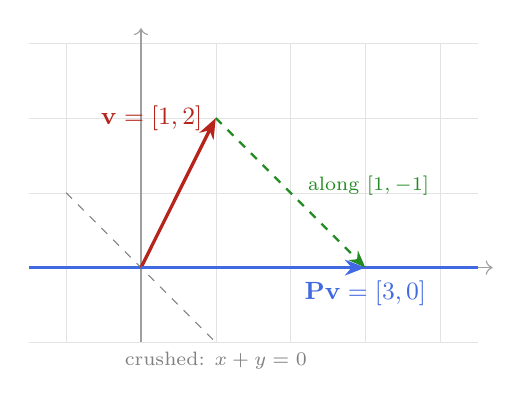
\begin{tikzpicture}[scale=0.95]
  \draw[step=1cm,gray!22,very thin] (-1.5,-1) grid (4.5,3);
  \draw[axisline] (-1.5,0) -- (4.7,0);
  \draw[axisline] (0,-1) -- (0,3.2);
  \draw[RoyalBlue,thick] (-1.5,0) -- (4.5,0);
  \draw[gray,dashed] (-1,1) -- (1,-1) node[below,font=\scriptsize]{crushed: $x+y=0$};
  \draw[vecarr,BrickRed] (0,0) -- (1,2);
  \node[left,font=\small,BrickRed] at (0.95,2) {$\vc{v}=[1,2]$};
  \draw[thinarr,ForestGreen,dashed] (1,2) -- (3,0);
  \draw[vecarr,RoyalBlue] (0,0) -- (3,0);
  \node[below,font=\small,RoyalBlue] at (3,-0.05) {$\mt{P}\vc{v}=[3,0]$};
  \node[right,font=\scriptsize,ForestGreen] at (2.1,1.1) {along $[1,-1]$};
\end{tikzpicture}
\end{center}

%------------------------------------------------------------------------------
\subsection{Orthogonal projections}
%------------------------------------------------------------------------------
What separates $\mt{P}_{\vc{u}}$ from the slanted example is symmetry:
$\mt{P}_{\vc{u}}\T=\mt{P}_{\vc{u}}$, while
$\begin{bmatrix}1&1\\0&0\end{bmatrix}$ is not symmetric.

\begin{defn}[Orthogonal projection matrix]
A square matrix $\mt{P}$ is an \textbf{orthogonal projection matrix} if
$\mt{P}^{2}=\mt{P}$ and $\mt{P}\T=\mt{P}$.
\end{defn}

\begin{thm}
\label{thm:orthproj}
If $\mt{P}$ is an orthogonal projection matrix, then for every $\vc{v}$ the
leftover $\vc{v}-\mt{P}\vc{v}$ is orthogonal to every vector of
$\colsp{\mt{P}}$.
\end{thm}

\begin{proof}
A vector of $\colsp{\mt{P}}$ has the form $\mt{P}\vc{w}$. Then
\[
  (\mt{P}\vc{w})\T(\vc{v}-\mt{P}\vc{v})
  =\vc{w}\T\mt{P}\T\vc{v}-\vc{w}\T\mt{P}\T\mt{P}\vc{v}
  =\vc{w}\T\mt{P}\vc{v}-\vc{w}\T\mt{P}^{2}\vc{v}
  =\vc{w}\T\mt{P}\vc{v}-\vc{w}\T\mt{P}\vc{v}=0,
\]
using $\mt{P}\T=\mt{P}$ and then $\mt{P}^{2}=\mt{P}$.
\end{proof}

\noindent So for an orthogonal projection the light falls perpendicular, which
is the picture of \S26.3 and the reason for the name. This theorem returns in
Part 9, where the best approximate solution of an unsolvable system turns out to
be an orthogonal projection.

%==============================================================================
\section{The complementary projection and reflections}
%==============================================================================

%------------------------------------------------------------------------------
\subsection{\texorpdfstring{$\mt{I}-\mt{P}$}{I - P} is a projection too}
%------------------------------------------------------------------------------
If $\mt{P}$ is a projection, so is $\mt{I}-\mt{P}$. By the distributive laws,
with $\mt{I}\mt{P}=\mt{P}\mt{I}=\mt{P}$,
\[
  (\mt{I}-\mt{P})^{2}=\mt{I}-2\mt{P}+\mt{P}^{2}=\mt{I}-2\mt{P}+\mt{P}=\mt{I}-\mt{P} .
\]
If $\mt{P}$ is symmetric, so is $\mt{I}-\mt{P}$, so the complement of an
orthogonal projection is an orthogonal projection. The matrix $\mt{I}-\mt{P}$ is
the \textbf{complementary projection}.

%------------------------------------------------------------------------------
\subsection{What it does}
%------------------------------------------------------------------------------
For the projection onto a line,
\[
  (\mt{I}-\mt{P}_{\vc{u}})\vc{v}=\vc{v}-\proj{\vc{u}}{\vc{v}},
\]
the orthogonal piece of the vector unit's \S12.6: the part of $\vc{v}$ that is
perpendicular to $\vc{u}$. The two projections split $\vc{v}$ between them:
\[
  \mt{P}_{\vc{u}}\vc{v}+(\mt{I}-\mt{P}_{\vc{u}})\vc{v}=\vc{v},
  \qquad
  \mt{P}_{\vc{u}}(\mt{I}-\mt{P}_{\vc{u}})=\mt{P}_{\vc{u}}-\mt{P}_{\vc{u}}^{2}=\mt{0},
  \qquad
  (\mt{I}-\mt{P}_{\vc{u}})\mt{P}_{\vc{u}}=\mt{0}.
\]
The pieces add back to $\vc{v}$, and each projection kills the other's piece.

%------------------------------------------------------------------------------
\subsection{In the plane: the projection onto the perpendicular line}
%------------------------------------------------------------------------------
In $\R^{2}$ the perpendicular piece lies on a single line: the line through a
vector $\vc{v}\perp\vc{u}$. Projecting onto that line is the same construction
as \S26 with $\vc{v}$ in the role of $\vc{u}$: the projection of any vector
$\vc{x}$ onto $\vc{v}$ is $\proj{\vc{v}}{\vc{x}}=\mt{P}_{\vc{v}}\vc{x}$, where
\[
  \mt{P}_{\vc{v}}=\frac{\vc{v}\vc{v}\T}{\vc{v}\T\vc{v}},
\]
the \textbf{orthogonal projection matrix with respect to $\vc{v}$}. The claim is
that this \emph{is} the complement of $\mt{P}_{\vc{u}}$.

\begin{thm}
\label{thm:complement}
Let $\vc{u}=[\,a,b\,]\neq\vc{0}$ and $\vc{v}=[\,-b,a\,]$, which is orthogonal to
$\vc{u}$ and has the same length. Then
\[
  \mt{P}_{\vc{u}}+\mt{P}_{\vc{v}}=\mt{I},
  \qquad\text{that is,}\qquad
  \mt{I}-\mt{P}_{\vc{u}}=\mt{P}_{\vc{v}} .
\]
\end{thm}

\begin{proof}
Add the two outer products:
\[
  \vc{u}\vc{u}\T+\vc{v}\vc{v}\T
  =\begin{bmatrix}a^{2}&ab\\ab&b^{2}\end{bmatrix}
   +\begin{bmatrix}b^{2}&-ab\\-ab&a^{2}\end{bmatrix}
  =(a^{2}+b^{2})\,\mt{I}.
\]
Both have denominator $\vc{u}\T\vc{u}=\vc{v}\T\vc{v}=a^{2}+b^{2}$, so dividing
gives $\mt{P}_{\vc{u}}+\mt{P}_{\vc{v}}=\mt{I}$.
\end{proof}

\begin{ex}
With $\vc{u}=[\,1,1\,]$ and $\vc{v}=[\,-1,1\,]$,
\[
  \mt{I}-\mt{P}_{\vc{u}}
  =\begin{bmatrix}1&0\\0&1\end{bmatrix}-\frac12\begin{bmatrix}1&1\\1&1\end{bmatrix}
  =\frac12\begin{bmatrix}1&-1\\-1&1\end{bmatrix}
  =\frac{\vc{v}\vc{v}\T}{\vc{v}\T\vc{v}}
  =\mt{P}_{\vc{v}} . \quad\checkmark
\]
\end{ex}

\begin{rmk}
In $\R^{3}$ the complement of a line projection is not a line projection: what
is perpendicular to $\vc{u}$ is a whole plane, and $\mt{I}-\mt{P}_{\vc{u}}$ has
rank $2$. With $\vc{u}=[\,1,1,1\,]$, $\mt{P}_{\vc{u}}$ replaces each entry by the
average (Example~\ref{ex:proj}(d)), so $\mt{I}-\mt{P}_{\vc{u}}$ subtracts the
average from each entry: $[\,1,2,6\,]\mapsto[\,-2,-1,3\,]$. Data scientists call
this \emph{centering}, and it is a projection onto the plane of vectors whose
entries sum to zero.
\end{rmk}

%------------------------------------------------------------------------------
\subsection{Reflection, from projection}
%------------------------------------------------------------------------------
A reflection across the line $\spanop\{\vc{u}\}$ keeps the piece of $\vc{v}$
along $\vc{u}$ and reverses the perpendicular piece:
\[
  \vc{v}\;\longmapsto\;\mt{P}_{\vc{u}}\vc{v}-(\mt{I}-\mt{P}_{\vc{u}})\vc{v}
  =(2\mt{P}_{\vc{u}}-\mt{I})\,\vc{v} .
\]
So the reflection across $\spanop\{\vc{u}\}$ is $2\mt{P}_{\vc{u}}-\mt{I}$, which
in the plane is also $\mt{P}_{\vc{u}}-\mt{P}_{\vc{v}}$. Check against Part 3:
$\vc{u}=\vc{e}_1$ gives $2\diagop(1,0)-\mt{I}=\diagop(1,-1)$, the reflection
across the $x$-axis, and $\vc{u}=[\,1,1\,]$ gives
$\begin{bmatrix}1&1\\1&1\end{bmatrix}-\mt{I}=\begin{bmatrix}0&1\\1&0\end{bmatrix}$,
the reflection across $y=x$.

It is symmetric, and $(2\mt{P}-\mt{I})^{2}=4\mt{P}^{2}-4\mt{P}+\mt{I}=\mt{I}$,
so it is its own transpose and squares to $\mt{I}$. Then
$(2\mt{P}-\mt{I})\T(2\mt{P}-\mt{I})=\mt{I}$, and it is an orthogonal matrix
(\S20.6): reflecting twice puts everything back, and lengths are kept.

%------------------------------------------------------------------------------
\subsection{Reflecting a vector onto the \texorpdfstring{$x$}{x}-axis}
%------------------------------------------------------------------------------
Here is a job for a reflection. Given a nonzero vector $\vc{u}\in\R^{2}$, find
a reflection that sends $\vc{u}$ onto the positive $x$-axis.

\medskip
\noindent\textbf{Where $\vc{u}$ must land.} A reflection keeps lengths
(\S28.4), so the image of $\vc{u}$ has length $\norm{\vc{u}}$. The only point
of the positive $x$-axis at that distance from the origin is
\[
  \norm{\vc{u}}\,\vc{e}_1=[\,\norm{\vc{u}},\,0\,].
\]

\noindent\textbf{Where the mirror must be.} A mirror line sits halfway between
a point and its reflection. So the midpoint of $\vc{u}$ and its image, which is
the \emph{average} (or centroid) of the two vectors,
\[
  \vc{m}=\frac{\vc{u}+\norm{\vc{u}}\,\vc{e}_1}{2},
\]
lies on the mirror. The mirror is a line through the origin, so it is
$\spanop\{\vc{m}\}$, as long as $\vc{m}\neq\vc{0}$ (\S28.7 handles the one
exception). There is a second way to see it. The vectors $\vc{u}$ and
$\norm{\vc{u}}\vc{e}_1$ have the same length, so the parallelogram they span is
a rhombus. Its diagonal $\vc{u}+\norm{\vc{u}}\vc{e}_1$ cuts the angle between
them in half, so the mirror is the line that bisects that angle.

\medskip
\noindent\textbf{A check.} The segment from $\vc{u}$ to its image should cross
the mirror at a right angle. It does, because the two vectors have the same
length:
\[
  (\vc{u}-\norm{\vc{u}}\vc{e}_1)\cdot(\vc{u}+\norm{\vc{u}}\vc{e}_1)
  =\vc{u}\cdot\vc{u}-\norm{\vc{u}}^{2}\,\vc{e}_1\cdot\vc{e}_1
  =\norm{\vc{u}}^{2}-\norm{\vc{u}}^{2}=0 .
\]
The picture is for $\vc{u}=[\,3,4\,]$, with $\norm{\vc{u}}=5$ and
$\vc{m}=\frac12\bigl([\,3,4\,]+[\,5,0\,]\bigr)=[\,4,2\,]$.

\begin{center}
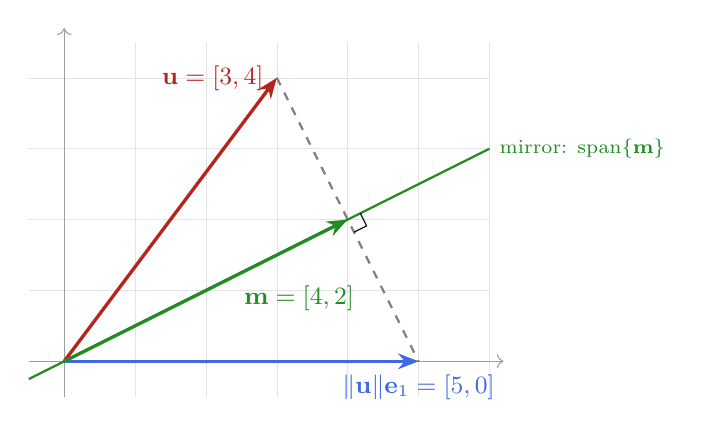
\begin{tikzpicture}[scale=0.9]
  \draw[step=1cm,gray!22,very thin] (-0.5,-0.5) grid (6,4.5);
  \draw[axisline] (-0.5,0) -- (6.2,0);
  \draw[axisline] (0,-0.5) -- (0,4.7);
  \draw[ForestGreen,thick] (-0.5,-0.25) -- (6,3)
       node[right,font=\scriptsize]{mirror: $\spanop\{\vc{m}\}$};
  \draw[dashed,thick,gray] (3,4) -- (5,0);
  \draw (4.179,2.089) -- (4.268,1.911) -- (4.089,1.821);
  \draw[vecarr,BrickRed] (0,0) -- (3,4);
  \node[left,font=\small,BrickRed] at (2.95,4) {$\vc{u}=[3,4]$};
  \draw[vecarr,RoyalBlue] (0,0) -- (5,0);
  \node[below,font=\small,RoyalBlue] at (5,-0.05) {$\norm{\vc{u}}\vc{e}_1=[5,0]$};
  \draw[vecarr,ForestGreen] (0,0) -- (4,2);
  \node[below right,font=\small,ForestGreen] at (2.4,1.2) {$\vc{m}=[4,2]$};
\end{tikzpicture}
\end{center}

%------------------------------------------------------------------------------
\subsection{The Householder reflector}
%------------------------------------------------------------------------------
Now build the reflection across $\spanop\{\vc{m}\}$ with \S28.4. Scale $\vc{m}$
to the unit vector $\vc{v}=\vc{m}/\norm{\vc{m}}$. Then
$\mt{P}_{\vc{m}}=\vc{v}\vc{v}\T$ (\S26.2), and the reflection is
$2\mt{P}_{\vc{m}}-\mt{I}$.

\needspace{12\baselineskip}
\begin{defn}[Householder reflector]
Let $\vc{u}\in\R^{2}$ be a nonzero vector that does not point along the negative
$x$-axis. Let
\[
  \vc{m}=\frac{\vc{u}+\norm{\vc{u}}\,\vc{e}_1}{2}
  \qquad\text{and}\qquad
  \vc{v}=\frac{\vc{m}}{\norm{\vc{m}}} .
\]
The \textbf{Householder reflector} for $\vc{u}$ is
\[
  \boxed{\;\mt{H}=2\vc{v}\vc{v}\T-\mt{I}_{2}\;},
\]
the reflection across the line spanned by the average of $\vc{u}$ and
$\norm{\vc{u}}\vc{e}_1$. Here $\mt{I}_{2}$ is the $2\times2$ identity.
\end{defn}

\begin{thm}
\label{thm:householder}
The Householder reflector sends $\vc{u}$ onto the positive $x$-axis:
$\mt{H}\vc{u}=\norm{\vc{u}}\,\vc{e}_1$.
\end{thm}

\begin{proof}
The key fact is that the projection of $\vc{u}$ onto the line through $\vc{m}$
is $\vc{m}$ itself. Write $r=\norm{\vc{u}}$, and $u_1=\vc{e}_1\cdot\vc{u}$ for the
first entry of $\vc{u}$. Then
\[
  \vc{m}\cdot\vc{u}
  =\tfrac12\bigl(\vc{u}\cdot\vc{u}+r\,\vc{e}_1\cdot\vc{u}\bigr)
  =\tfrac12\bigl(r^{2}+ru_1\bigr),
\]
\[
  \vc{m}\cdot\vc{m}
  =\tfrac14\bigl(\vc{u}\cdot\vc{u}+2r\,\vc{e}_1\cdot\vc{u}
     +r^{2}\,\vc{e}_1\cdot\vc{e}_1\bigr)
  =\tfrac14\bigl(2r^{2}+2ru_1\bigr)
  =\tfrac12\bigl(r^{2}+ru_1\bigr).
\]
The two are equal, so
$\mt{P}_{\vc{m}}\vc{u}=\frac{\vc{m}\cdot\vc{u}}{\vc{m}\cdot\vc{m}}\,\vc{m}=\vc{m}$.
Therefore
\[
  \mt{H}\vc{u}=2\mt{P}_{\vc{m}}\vc{u}-\vc{u}
  =2\vc{m}-\vc{u}
  =(\vc{u}+r\,\vc{e}_1)-\vc{u}
  =r\,\vc{e}_1 .
  \qedhere
\]
\end{proof}

\noindent In the language of \S28.4, the piece of $\vc{u}$ along the mirror is
$\vc{m}$, and the perpendicular piece is
$\vc{u}-\vc{m}=\frac12(\vc{u}-\norm{\vc{u}}\vc{e}_1)$. The reflection keeps the
first piece and reverses the second, which gives
$\vc{m}-(\vc{u}-\vc{m})=2\vc{m}-\vc{u}$.

\begin{ex}
\label{ex:householder}
Take $\vc{u}=[\,3,4\,]$, as in the picture of \S28.5. There
$\vc{m}=[\,4,2\,]$, so $\norm{\vc{m}}=\sqrt{20}$ and
$\vc{v}=\frac{1}{\sqrt{20}}[\,4,2\,]=\frac{1}{\sqrt5}[\,2,1\,]$. Then
$\vc{v}\vc{v}\T=\frac15\begin{bmatrix}4&2\\2&1\end{bmatrix}$, the projection
onto the line through $[\,2,1\,]$ from Example~\ref{ex:proj}(c), and
\[
  \mt{H}=\frac25\begin{bmatrix}4&2\\2&1\end{bmatrix}
        -\begin{bmatrix}1&0\\0&1\end{bmatrix}
  =\frac15\begin{bmatrix}3&4\\4&-3\end{bmatrix},
  \qquad
  \mt{H}\vc{u}=\frac15\,[\,9+16,\ 12-12\,]=[\,5,0\,] . \quad\checkmark
\]
\end{ex}

%------------------------------------------------------------------------------
\subsection{Properties, and the usual form}
%------------------------------------------------------------------------------
\textbf{It is a reflection.} $\mt{H}$ is built as in \S28.4, so it is
symmetric, $\mt{H}^{2}=\mt{I}$, and it is orthogonal. Its determinant is $-1$:
in Example~\ref{ex:householder}, $\frac{1}{25}(-9-16)=-1$.

\medskip
\noindent\textbf{Its first column is $\vc{u}$, scaled to length $1$.} Apply
$\mt{H}$ to both sides of $\mt{H}\vc{u}=\norm{\vc{u}}\vc{e}_1$. Since
$\mt{H}^{2}=\mt{I}$, this gives $\vc{u}=\norm{\vc{u}}\,\mt{H}\vc{e}_1$, so
$\mt{H}\vc{e}_1=\vc{u}/\norm{\vc{u}}$. Every $2\times2$ orthogonal matrix with
determinant $-1$ has the form $\begin{bmatrix}a&c\\c&-a\end{bmatrix}$ (\S21.2),
so in the plane
\[
  \mt{H}=\frac{1}{\norm{\vc{u}}}\begin{bmatrix}u_1&u_2\\u_2&-u_1\end{bmatrix}.
\]
This is a quick check on a computation. In Example~\ref{ex:householder} it reads
$\frac15\begin{bmatrix}3&4\\4&-3\end{bmatrix}$. It is not a replacement for the
construction, since it works only in the plane.

\medskip
\noindent\textbf{The exception.} If $\vc{u}$ points along the negative
$x$-axis, then $\vc{u}=-\norm{\vc{u}}\vc{e}_1$ and the average $\vc{m}$ is
$\vc{0}$, so there is no line to reflect across. No construction is needed:
the reflection across the $y$-axis, $\diagop(-1,1)$, sends $\vc{u}$ to
$\norm{\vc{u}}\vc{e}_1$.

\medskip
\noindent\textbf{The usual form.} Software, and most books, write a Householder
reflector as $\mt{I}-2\vc{w}\vc{w}\T$ with $\vc{w}$ a unit vector. In the plane
this is the same matrix. Take $\vc{w}$ to be a unit vector perpendicular to
$\vc{v}$. Theorem~\ref{thm:complement} gives
$\vc{v}\vc{v}\T+\vc{w}\vc{w}\T=\mt{I}$, so
\[
  2\vc{v}\vc{v}\T-\mt{I}
  =2(\mt{I}-\vc{w}\vc{w}\T)-\mt{I}
  =\mt{I}-2\vc{w}\vc{w}\T .
\]
By the check in \S28.5, $\vc{w}$ points along $\vc{u}-\norm{\vc{u}}\vc{e}_1$, the
segment from the image to $\vc{u}$. So $\mt{I}-2\vc{w}\vc{w}\T$ reads ``reflect
across the line perpendicular to $\vc{w}$''. That description carries over to
$\R^{n}$: there the vectors perpendicular to $\vc{w}$ form an
$(n-1)$-dimensional subspace (a plane, in $\R^{3}$), and
$\mt{I}-2\vc{w}\vc{w}\T$ reflects across it. The reflectors are named for Alston
Householder, who introduced them for this purpose in 1958.

\lookahead Part 11 uses a sequence of Householder reflectors to compute the
$QR$ decomposition. Each one turns a column into a multiple of $\vc{e}_1$,
which zeros out every entry below the first, and keeps lengths exactly.

%==============================================================================
\section{The direct sum}
%==============================================================================

%------------------------------------------------------------------------------
\subsection{Splitting a vector}
%------------------------------------------------------------------------------
Take orthogonal nonzero vectors $\vc{u}$ and $\vc{v}$ in $\R^{2}$. By
Theorem~\ref{thm:complement}, every $\vc{x}\in\R^{2}$ splits as
\[
  \vc{x}=\mt{P}_{\vc{u}}\vc{x}+\mt{P}_{\vc{v}}\vc{x},
  \qquad
  \mt{P}_{\vc{u}}\vc{x}\in\spanop\{\vc{u}\},\quad
  \mt{P}_{\vc{v}}\vc{x}\in\spanop\{\vc{v}\} :
\]
a piece on each line.

\begin{ex}
\label{ex:split}
With $\vc{u}=[\,1,1\,]$, $\vc{v}=[\,-1,1\,]$ and $\vc{x}=[\,3,1\,]$:
$\mt{P}_{\vc{u}}\vc{x}=[\,2,2\,]$ and
$\mt{P}_{\vc{v}}\vc{x}=\frac12[\,2,-2\,]=[\,1,-1\,]$. Their sum is $[\,3,1\,]$.
\end{ex}

%------------------------------------------------------------------------------
\subsection{The split is unique}
%------------------------------------------------------------------------------
More is true: there is \emph{no other way} to write $\vc{x}$ as a vector on the
first line plus a vector on the second. Suppose
$\vc{x}=\vc{p}+\vc{q}=\vc{p}'+\vc{q}'$, with $\vc{p},\vc{p}'$ on
$\spanop\{\vc{u}\}$ and $\vc{q},\vc{q}'$ on $\spanop\{\vc{v}\}$. Then
\[
  \vc{p}-\vc{p}'=\vc{q}'-\vc{q}
\]
is a vector on both lines. Two different lines through the origin meet only at
the origin, since $\vc{u}$ and $\vc{v}$ are independent (the vector unit,
\S21.2) and $c\vc{u}=d\vc{v}$ forces $c=d=0$. So $\vc{p}=\vc{p}'$ and
$\vc{q}=\vc{q}'$.

%------------------------------------------------------------------------------
\subsection{The definition}
%------------------------------------------------------------------------------
\begin{defn}[Direct sum]
Let $U$ and $W$ be subspaces of a subspace $V$. Then $V$ is the \textbf{direct
sum} of $U$ and $W$, written
\[
  V=U\oplus W,
\]
if every vector of $V$ can be written in exactly one way as $\vc{u}+\vc{w}$ with
$\vc{u}\in U$ and $\vc{w}\in W$.
\end{defn}

\noindent Two things are being asked: that every vector \emph{can} be split
(the subspaces together reach everything), and that the split is
\emph{unique}. The second can be replaced by a simpler test.

\begin{thm}
\label{thm:directsum}
$V=U\oplus W$ if and only if every vector of $V$ is a sum $\vc{u}+\vc{w}$ with
$\vc{u}\in U$, $\vc{w}\in W$, and $U\cap W=\{\vc{0}\}$.
\end{thm}

\begin{proof}
If $U\cap W=\{\vc{0}\}$, the argument of \S29.2 shows splittings are unique.
Conversely, if some $\vc{z}\neq\vc{0}$ lay in both, then
$\vc{0}=\vc{0}+\vc{0}=\vc{z}+(-\vc{z})$ would be two different splittings of
$\vc{0}$.
\end{proof}

\noindent So, for orthogonal nonzero $\vc{u},\vc{v}$,
\[
  \R^{2}=\spanop\{\vc{u}\}\oplus\spanop\{\vc{v}\},
\]
and the two projections $\mt{P}_{\vc{u}}$ and $\mt{P}_{\vc{v}}=\mt{I}-\mt{P}_{\vc{u}}$
are the machines that find the two pieces. Because the pieces are orthogonal,
their lengths obey the Pythagorean identity (the vector unit, \S23):
\[
  \norm{\vc{x}}^{2}=\norm{\mt{P}_{\vc{u}}\vc{x}}^{2}+\norm{\mt{P}_{\vc{v}}\vc{x}}^{2}.
\]
In Example~\ref{ex:split}, $10=8+2$.

\begin{center}
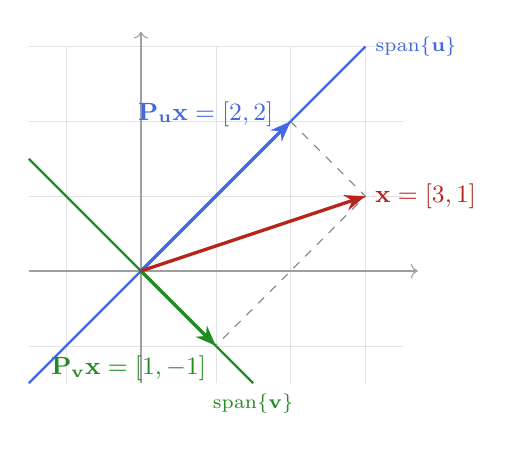
\begin{tikzpicture}[scale=0.95]
  \draw[step=1cm,gray!22,very thin] (-1.5,-1.5) grid (3.5,3);
  \draw[axisline] (-1.5,0) -- (3.7,0);
  \draw[axisline] (0,-1.5) -- (0,3.2);
  \draw[RoyalBlue,thick] (-1.5,-1.5) -- (3,3) node[right,font=\scriptsize]{$\spanop\{\vc{u}\}$};
  \draw[ForestGreen,thick] (-1.5,1.5) -- (1.5,-1.5) node[below,font=\scriptsize]{$\spanop\{\vc{v}\}$};
  \draw[vecarr,RoyalBlue] (0,0) -- (2,2);
  \draw[vecarr,ForestGreen] (0,0) -- (1,-1);
  \draw[dashed,gray] (2,2) -- (3,1) -- (1,-1);
  \draw[vecarr,BrickRed] (0,0) -- (3,1);
  \node[right,font=\small,BrickRed] at (3,1) {$\vc{x}=[3,1]$};
  \node[left,font=\small,RoyalBlue] at (1.9,2.1) {$\mt{P}_{\vc{u}}\vc{x}=[2,2]$};
  \node[below left,font=\small,ForestGreen] at (1,-1) {$\mt{P}_{\vc{v}}\vc{x}=[1,-1]$};
\end{tikzpicture}
\end{center}

%------------------------------------------------------------------------------
\subsection{Direct sums need not be orthogonal}
%------------------------------------------------------------------------------
Nothing in the definition mentions angles. The slanted projection of \S27.3,
$\mt{P}=\begin{bmatrix}1&1\\0&0\end{bmatrix}$, and its complement
$\mt{I}-\mt{P}=\begin{bmatrix}0&-1\\0&1\end{bmatrix}$ split
$\vc{x}=[\,x,y\,]$ as
\[
  \vc{x}=\underbrace{[\,x+y,\ 0\,]}_{\text{on the }x\text{-axis}}
        +\underbrace{[\,-y,\ y\,]}_{\text{on }\spanop\{[-1,1]\}},
\]
so $\R^{2}=\spanop\{[\,1,0\,]\}\oplus\spanop\{[\,-1,1\,]\}$, two lines at
$135^\circ$. For $\vc{x}=[\,3,1\,]$ the pieces are $[\,4,0\,]$ and $[\,-1,1\,]$.
They are not orthogonal, and the Pythagorean identity fails: $10\neq16+2$. A
direct sum needs only that the two subspaces reach everything and meet only at
$\vc{0}$; orthogonality is an extra, and a valuable one.

%------------------------------------------------------------------------------
\subsection{Every projection splits the space}
%------------------------------------------------------------------------------
The pattern is general. For any projection $\mt{P}\in\R^{n\times n}$,
\[
  \R^{n}=\colsp{\mt{P}}\oplus\colsp{\mt{I}-\mt{P}} .
\]
Every $\vc{x}$ splits as $\mt{P}\vc{x}+(\mt{I}-\mt{P})\vc{x}$, a vector of each.
And the two meet only at $\vc{0}$: if $\vc{z}=\mt{P}\vc{a}=(\mt{I}-\mt{P})\vc{b}$,
then on one hand $\mt{P}\vc{z}=\mt{P}^{2}\vc{a}=\mt{P}\vc{a}=\vc{z}$, and on the
other $\mt{P}\vc{z}=\mt{P}(\mt{I}-\mt{P})\vc{b}=\vc{0}$, so $\vc{z}=\vc{0}$.
Conversely, given any direct sum $\R^{n}=U\oplus W$, the rule ``keep the
$U$-piece'' is linear and idempotent, so it is a projection. Projections and
direct sums are two descriptions of the same thing.

\begin{ex}
In $\R^{3}$, with $\vc{u}=[\,1,1,1\,]$,
$\R^{3}=\spanop\{\vc{u}\}\oplus\{\vc{x}:x_1+x_2+x_3=0\}$, a line and the plane
perpendicular to it. The vector $[\,1,2,6\,]$ splits as
$[\,3,3,3\,]+[\,-2,-1,3\,]$, its average and its centered part.
\end{ex}

%------------------------------------------------------------------------------
\subsection{Practice}
%------------------------------------------------------------------------------
\begin{enumerate}[label=\textbf{P\arabic*.},leftmargin=2.6em,itemsep=5pt]
  \item Write $\mt{P}_{\vc{u}}$ for $\vc{u}=[\,3,4\,]$, and use it to project
        $[\,1,0\,]$ and $[\,4,-3\,]$.
  \item Which of these are projection matrices, and which are orthogonal
        projection matrices?
        \[
          \begin{bmatrix}0&0\\0&1\end{bmatrix},\qquad
          \begin{bmatrix}1&0\\1&0\end{bmatrix},\qquad
          \begin{bmatrix}\tfrac12&\tfrac12\\[2pt]\tfrac12&\tfrac12\end{bmatrix},\qquad
          \begin{bmatrix}2&0\\0&0\end{bmatrix}.
        \]
  \item For $\vc{u}=[\,1,2\,]$, compute $\mt{I}-\mt{P}_{\vc{u}}$ and check that it
        equals $\mt{P}_{\vc{v}}$ with $\vc{v}=[\,-2,1\,]$.
  \item With the same $\vc{u}$ and $\vc{v}$, split $\vc{x}=[\,4,3\,]$ into a piece
        on each line and check the Pythagorean identity.
  \item Find the matrix of the reflection across the line through $[\,1,2\,]$,
        and reflect $[\,1,0\,]$.
  \item Show that if $\mt{P}$ is a projection then $\mt{P}^{k}=\mt{P}$ for every
        $k\ge1$.
  \item Find the Householder reflector $\mt{H}$ for $\vc{u}=[\,-3,4\,]$. Check
        that $\mt{H}\vc{u}=[\,5,0\,]$ and that the first column of $\mt{H}$ is
        $\vc{u}/\norm{\vc{u}}$. Compare with P5.
\end{enumerate}

\subsubsection*{Answers}

\noindent\textbf{P1.} $\mt{P}_{\vc{u}}=\frac{1}{25}\begin{bmatrix}9&12\\12&16\end{bmatrix}$.
$[\,1,0\,]\mapsto\frac{1}{25}[\,9,12\,]$, and $[\,4,-3\,]\mapsto\vc{0}$, since
$[\,4,-3\,]\perp[\,3,4\,]$.

\smallskip
\noindent\textbf{P2.} $\diagop(0,1)$: idempotent and symmetric, orthogonal
projection onto the $y$-axis. $\begin{bmatrix}1&0\\1&0\end{bmatrix}$: its square
is itself, so it is a projection, but it is not symmetric. It sends $[\,x,y\,]$
to $[\,x,x\,]$, onto the line $y=x$ along vertical lines, a slanted one.
$\frac12\begin{bmatrix}1&1\\1&1\end{bmatrix}=\mt{P}_{[1,1]}$: orthogonal
projection. $\diagop(2,0)$: its square is $\diagop(4,0)$, not a projection.

\smallskip
\noindent\textbf{P3.} $\mt{P}_{\vc{u}}=\frac15\begin{bmatrix}1&2\\2&4\end{bmatrix}$,
so $\mt{I}-\mt{P}_{\vc{u}}=\frac15\begin{bmatrix}4&-2\\-2&1\end{bmatrix}$, and
$\vc{v}\vc{v}\T/\vc{v}\T\vc{v}=\frac15\begin{bmatrix}4&-2\\-2&1\end{bmatrix}$.
\checkmark

\smallskip
\noindent\textbf{P4.} $\mt{P}_{\vc{u}}\vc{x}=\frac{4+6}{5}[\,1,2\,]=[\,2,4\,]$ and
$\mt{P}_{\vc{v}}\vc{x}=\frac{-8+3}{5}[\,-2,1\,]=[\,2,-1\,]$. Sum $[\,4,3\,]$;
$25=20+5$. \checkmark

\smallskip
\noindent\textbf{P5.} $2\mt{P}_{\vc{u}}-\mt{I}=\frac25\begin{bmatrix}1&2\\2&4\end{bmatrix}-\mt{I}
=\begin{bmatrix}-\frac35&\frac45\\[2pt]\frac45&\frac35\end{bmatrix}$, and
$[\,1,0\,]\mapsto[\,-\tfrac35,\tfrac45\,]$. (A reflection of the form
$\begin{bmatrix}a&c\\c&-a\end{bmatrix}$, as \S21 requires.)

\smallskip
\noindent\textbf{P6.} By induction: $\mt{P}^{k+1}=\mt{P}^{k}\mt{P}=\mt{P}\mt{P}=\mt{P}$.

\smallskip
\noindent\textbf{P7.} $\norm{\vc{u}}=5$, so
$\vc{m}=\frac12\bigl([\,-3,4\,]+[\,5,0\,]\bigr)=[\,1,2\,]$ and
$\vc{v}=\frac{1}{\sqrt5}[\,1,2\,]$. Then
\[
  \mt{H}=\frac25\begin{bmatrix}1&2\\2&4\end{bmatrix}-\mt{I}
  =\begin{bmatrix}-\frac35&\frac45\\[2pt]\frac45&\frac35\end{bmatrix},
  \qquad
  \mt{H}\vc{u}=\Bigl[\,\frac{9+16}{5},\ \frac{-12+12}{5}\,\Bigr]=[\,5,0\,].
\]
The first
column is $[\,-\frac35,\frac45\,]=\vc{u}/5$. \checkmark\ It is the matrix of P5:
the mirror is the line through $[\,1,2\,]$, and P5's
$[\,1,0\,]\mapsto[\,-\frac35,\frac45\,]$ is the first-column fact,
$\mt{H}\vc{e}_1=\vc{u}/\norm{\vc{u}}$.

\lookahead Part 6 takes the two subspaces that a projection splits the space
into, $\colsp{\mt{P}}$ and what $\mt{P}$ crushes, and asks the same questions of
every matrix. What does it reach? What does it crush to $\vc{0}$? The second set
is the null space, and the rank--nullity theorem says how the two sizes are
related.

\end{document}
